\apendice{Documentación técnica de programación}

\section{Introducción}
Este capítulo es fundamental para una posible evolución y mantenimiento del proyecto. En este se va a detallar la estructura de directorios del proyecto y un manual para futuros programadores del proyecto el cual incluye las directrices para realizar la compilación, instalación y ejecución de este. Además, de expondrán cuales han sido los test implementados y de qué manera se han implementado los mismos.
\section{Estructura de directorios}
El repositorio de proyecto en GitHub, al cual se puede acceder mediante el siguiente \href{https://github.com/miguelUbierna/DeltaOffers}{enlace}, tiene los siguientes principales directorios:

\begin{itemize}
    \item \texttt{.github:} El cual tiene en su interior un directorio \texttt{workflows} en el que aparecerán los archivos de extensión \textit{.yml} utilizados para definir flujos de trabajo en GitHub Actions. En este caso, estos serán los encargados de actualizar la base de datos del sistema de manera periódica. La estructura de este directorio, no se volverá a explicar previamente dado que ha sido explicada en este punto.
    \item \textbf{DataCollections:} Este es el directorio que contiene el proyecto en Python. En él se realiza el \textit{web scraping}, la actualización de la base de datos y las pruebas unitarias.
    \item \textbf{DeltaOffersWeb:} Incluye el proyecto .NET Core MVC en el que se desarrolla la aplicación web con la que el usuario podrá interaccionar y en la que se muestran las convocatorias de manera centralizada.
    \item \textbf{Doc:} En este directorio residirá la documentación del proyecto. Esta documentación ha sido realizada con Latex y contiene dos partes: la memoria y los anexos.
\end{itemize}
A continuación, se va a detallar cual es la estructura de directorios interna contenida dentro de los directorios principales mencionados anteriormente:

\subsection{DataCollections:}

Estructura del directorio DataCollecions:
\begin{itemize}
    \item \textbf{Data:} Contiene los \textit{scripts} que llaman a las clases que realizan el \textit{scraping} y actualizan la base de datos.
    \item \textbf{Images:} Incluye imágenes de logos que van a ser introducidos en la base de datos.
    \item \textbf{Interfaces:} Directorio con interfaz de la que van a heredar las clases concretas en las que se realiza el \textit{scraping} de cada universidad.
    \item \textbf{Scrapers:} Directorio en el que se encuentran las carpetas las cuales tienen en su interior las clases donde se implementa la lógica del \textit{web scraping} de cada universidad.
    \begin{itemize}
        \item \textbf{Scrapers/ScrapingUBU} : lógica web scraping UBU.
        \item \textbf{Scrapers/ScrapingUVA} : lógica web scraping UVA.
        \item \textbf{Scrapers/ScrapingULE} : lógica web scraping ULE.
    \end{itemize}
    \item \textbf{Test:} Contiene los \textit{scripts} de las pruebas unitarias realizadas para cada una de las universidades.
\end{itemize}

\subsection{DeltaOffersWeb:}

Estructura del directorio DeltaOffersWeb:
\begin{itemize}
    \item \textbf{Dependencies:} Incluye todas las dependencias utilizadas en la aplicación.
    \item \textbf{Properties:} En él se indican los perfiles de lanzamiento de la aplicación.
    \item \textbf{wwwroot:} Contiene distintos directorios dentro con los archivos estáticos utilizados. En estos archivos estáticos podemos encontrar:
    \begin{itemize}
        \item Archivos CSS para estilos del proyecto.
        \item Archivos JavaScript que incluye lógica y animaciones utilizadas.
        \item Imágenes utilizadas en la web
        \item Otros como bootstap, jquery, etc
    \end{itemize}
    \item \textbf{Controllers:} Aparecen los controladores que gestionan la lógica de negocio y que pasan datos a la vista.
    \item \textbf{Models:} Incluye el contexto (capa de abstracción entre la base de datos y el código) y las clases utilizadas como acceso a los datos.
    \item \textbf{ViewModels:} Contiene las clases utilizadas para pasar datos específicos a la vista.
    \item \textbf{Views:} Contiene vistas con las que interactúa el usuario. Este directorio contiene los siguientes en su interior:
    \begin{itemize}
        \item \textbf{Detalle:} Reside el código de las vistas para las ventanas de detalles.
        \item \textbf{Home:} Contiene el código de la vista inicial
        \item \textbf{Universidad:} Reside el código de las vistas para las ventanas de detalles.
        \item \textbf{Shared:} Contiene el código de componentes compartidos que aparecen en todas las ventanas como el encabezado de la aplicación.
    \end{itemize}  
\end{itemize}

\subsection{Docs:}

Estructura del directorio Docs:
\begin{itemize}
    \item \textbf{img: } Contiene las imágenes incluidas en la documentación.
    \item \textbf{tex: } Incluye los archivos .tex con los correspondientes capítulos de la memoria y los anexos.
\end{itemize}
    
\section{Manual del programador}
En este manual se van a dar las directivas necesarias para que nuevos desarrolladores puedan trabajar con la aplicación, aportar nuevas funcionalidades o mejorar su usabilidad. Para ello se van a describir cual es el proceso de montaje del proyecto desde la instalación de herramientas hasta la ejecución del mismo.

\subsection{Git:} En primer lugar, dado que el código del proyecto está alojado en un repositorio de GitHub, los usuarios tendrán que proceder a la instalación de Git. Esta es una herramienta utilizada para el control de versiones y que permite que diferentes usuarios puedan bajarse el código a sus equipos para trabajar con el de manera local. Para realizar esta labor una vez que tenemos Git instalado deberemos colocarnos en el directorio en el que deseamos que se aloje nuestro proyecto en local y ejecutar desde la terminal lo siguiente:

\texttt{git clone https://github.com/miguelUbierna/DeltaOffers}
\begin{figure}[H]
    \centering
    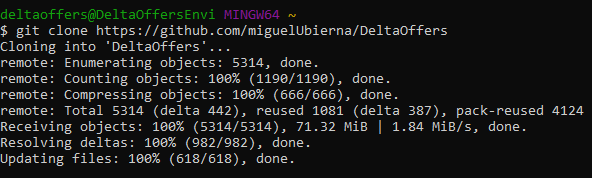
\includegraphics[width=0.8\linewidth]{DocumentacionTFG//img/GitClone.PNG}
    \caption{Ejecución Git clone}
\end{figure}

Tal y como se puede apreciar en la imagen, el comando \textit{git clone} irá seguido de la URL en la cual se puede encontrar el repositorio de GitHub. Posteriormente, podemos comprobar que el directorio del proyecto ya lo tenemos en nuestro equipo para trabajar con él de manera local.

\begin{figure}[H]
    \centering
    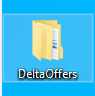
\includegraphics[width=0.15\linewidth]{DocumentacionTFG//img/DirectorioProyecto.PNG}
    \caption{Directorio del proyecto}
\end{figure}

\subsection{MySQL Server y MySQL Workbench}
Este proyecto consiste en la recopilación de datos de páginas web de las universidades mediante \textit{web scraping}. Estos datos recolectados, deberán almacenarse de manera segura y estructurada. Para lograr esto, se decidió utilizar una base de datos MySQL y por lo tanto se necesitaron instalar unas herramientas para el uso de este tipo de base de datos.

En primer lugar, el usuario debe instalar MySQL Server, esta herramienta se trata de un software gestor de bases de datos relacionales muy potente. Gracias a ella, nuestro equipo local funcionará como un servidor y gestor de bases de datos.

Posteriormente, se procede a la instalación de MySQL Workbench. Esta herramienta nos permitirá la creación de bases de datos, tablas y ejecución de consultas de una manera sencilla. Una vez instalada, se debe crear una nueva conexión con el servidor MySQL y crear la nueva base de datos junto con las siguientes tablas:

\begin{figure}[H]
    \centering
    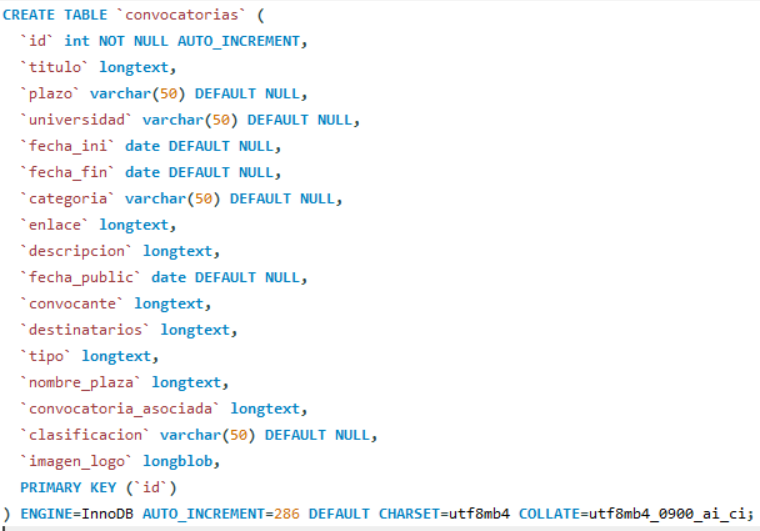
\includegraphics[width=0.8\linewidth]{DocumentacionTFG//img/CreacionTablaConvocatorias.PNG}
    \caption{Tabla Convocatorias}
\end{figure}

\begin{figure}[H]
    \centering
    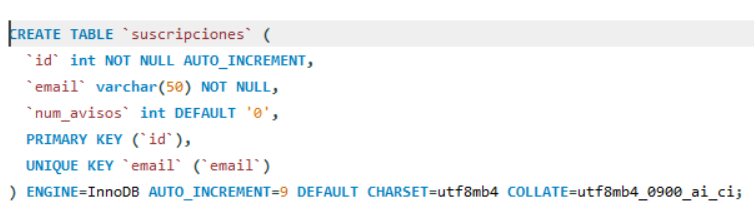
\includegraphics[width=0.8\linewidth]{DocumentacionTFG//img/CreacionTablaSuscripciones.PNG}
    \caption{Tabla Suscripciones}
\end{figure}

Con la creación de tablas ya realizada. Tan solo se volverá a utilizar esta herramienta para comprobar que los datos recopilados mediante \textit{web scraping} y cargados en la base de datos son los correctos.

\subsection{Instalación entorno proyecto Python}
Para la realización del web scraping y la actualización de la base de datos creada anteriormente, se utilizó el lenguaje de programación Python. En esta subsección se van a detallar los pasos a seguir para poder ejecutar este proyecto y que se actualice la base de datos con los datos recopilados.

En primer lugar, es necesario un entorno de desarrollo. Como editor de código, en este caso fue utilizado Visual Studio Code y por lo tanto como paso inicial es fundamental la instalación de esta herramienta, lo cual se puede realizar a través del siguiente \href{https://code.visualstudio.com/download}{enlace}. Una vez instalado Visual Studio Code, realizaremos también la instalación de la extensión de Python disponible para este editor.

\begin{figure}[H]
    \centering
    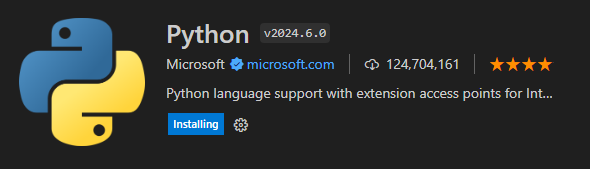
\includegraphics[width=0.75\linewidth]{DocumentacionTFG//img/ExtensionPythonVsCode.PNG}
    \caption{Extensión Python Visual Studio Code}
\end{figure}

Posteriormente, se descargará Python desde la web oficial, concretamente la versión \textit{3.12.2} que es la versión utilizada en el proyecto. Para la utilización de esta herramienta, será necesario modificar las variables de entorno del sistema añadiendo las siguientes rutas:

\begin{figure}[H]
    \centering
    \includegraphics[width=0.85\linewidth]{DocumentacionTFG//img/¨VariableEntornoPython.PNG}
    \caption{Variables de Entorno Python}
\end{figure}


Finalizado este proceso, podemos abrir el proyecto en Python (el repositorio DataCollections) con esta herramienta para poder comenzar con el trabajo.

\begin{figure}[H]
    \centering
    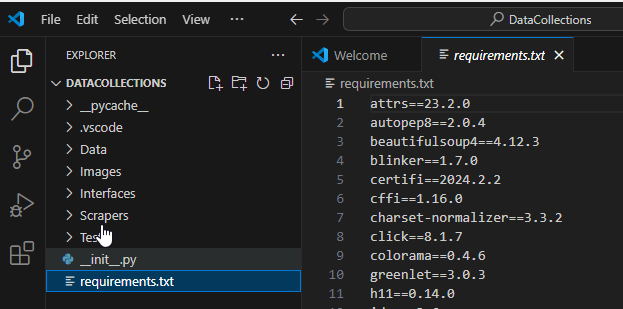
\includegraphics[width=0.85\linewidth]{DocumentacionTFG//img/VsCode.PNG}
    \caption{Proyecto Python Visual Studio Code}
    \label{fig:proyecto-vscode}
\end{figure}

Si intentamos ejecutar el proyecto, podemos apreciar que nos aparecerán errores debido a que no se han instalado los módulos necesarios. Todas estas dependencias, aparecerán en un fichero \textit{requirements.txt} tal y como aparece en la imagen \ref{fig:proyecto-vscode}, para instalarlas debemos ejecutar en la terminal de Visual Studio Code lo siguiente:

\begin{figure}[H]
    \centering
    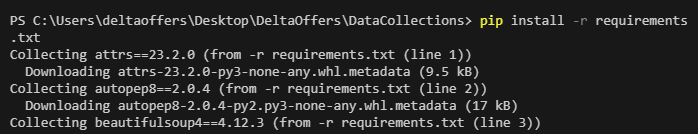
\includegraphics[width=1\linewidth]{DocumentacionTFG//img/IntalacionDependenciasPython.PNG}
    \caption{Instalación dependencias}
\end{figure}

Para que al ejecutar el proyecto se actualice la base de datos, tenemos que conectarnos con la misma. Para ello, indicaremos en el código en Python, cual es el \textit{host} al que queremos conectarnos, el usuario, la contraseña y el nombre de la base de datos.
\begin{figure}[H]
    \centering
    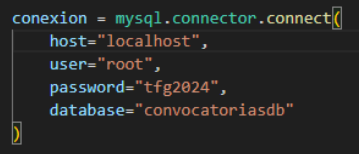
\includegraphics[width=0.5\linewidth]{DocumentacionTFG//img/ConnectionStringPython.PNG}
    \caption{Conexión Python con la base de datos MySQL}
\end{figure}


Pare ejecutar el proyecto, iremos al fichero \textit{data.py} haremos \textit{click} derecho sobre él y elegiremos la opción \textit{'Run Python/ Run Python File in Terminal'}. De esta manera se comenzará con la ejecución. Dado que el \textit{web scraping} es un proceso de extracción de datos extenso en el que se tienen que hacer peticiones HTTP, este proceso puede tardar unos minutos. Finalizado ese tiempo podremos ver ya la base de datos MySQL actualizada con la recopilación de las correspondientes convocatorias.

\begin{figure}[H]
    \centering
    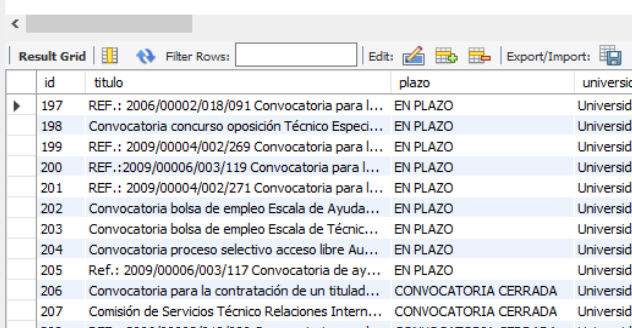
\includegraphics[width=0.9\linewidth]{DocumentacionTFG//img/ConvocatoriasEnBdLocal.PNG}
    \caption{Convocatorias insertadas en la base de datos}
\end{figure}

\subsection{Instalación entorno aplicación .NET}
Este será el último paso que debemos de realizar para que nuestro proyecto funcione de manera local. En primer lugar, debemos realizar la instalación de Visual Studio Community, herramienta, la cual puede instalarse a través del siguiente \href{https://visualstudio.microsoft.com/es/vs/community/}{enlace}.

Una vez realizado esto, en el instalador de Visual Studio, cargaremos las librerías necesarias para el desarrollo de ASP.NET y web. Para ello marcaremos la siguiente opción.
\begin{figure}[H]
    \centering
    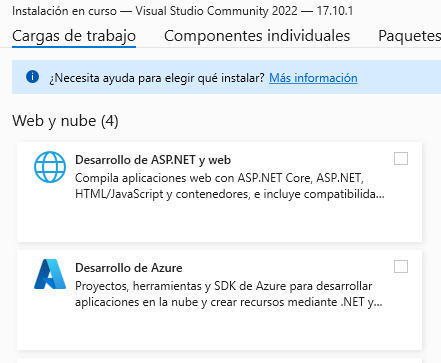
\includegraphics[width=0.75\linewidth]{DocumentacionTFG//img/InstaladorVisualStudio.PNG}
    \caption{Cargas de trabajo Visual Studio Community}
\end{figure}

Finalizado lo anterior, podemos abrir nuestra aplicación de Visual Studio y cargar el proyecto desarrollado en .NET Core el cual está alojado en el directorio 'DeltaOffersWeb' dentro del respositorio general del proyecto.

Una vez abierto, debemos configurar la cadena de conexión desde el fichero \textit{AppSettings.json} para que nuestra aplicación obtenga la información de la base de datos MySQL preparada previamente. La cadena de conexión quedará definida de la siguiente manera:

\begin{figure}[H]
    \centering
    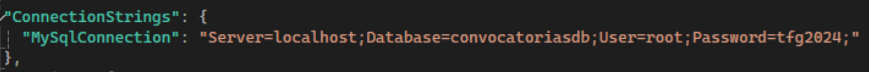
\includegraphics[width=1\linewidth]{DocumentacionTFG//img/ConnectionStringNet.PNG}
    \caption{Cadena de conexión .NET}
\end{figure}

Habiendo completado los pasos anteriores, ya podremos ejecutar la aplicación. Para ello bastará con pulsar el botón \textit{'Play'} en Visual Studio. Una vez realizado esto ya podemos ver la aplicación funcionando de manera local y estará disponible para su uso.

\begin{figure}[H]
    \centering
    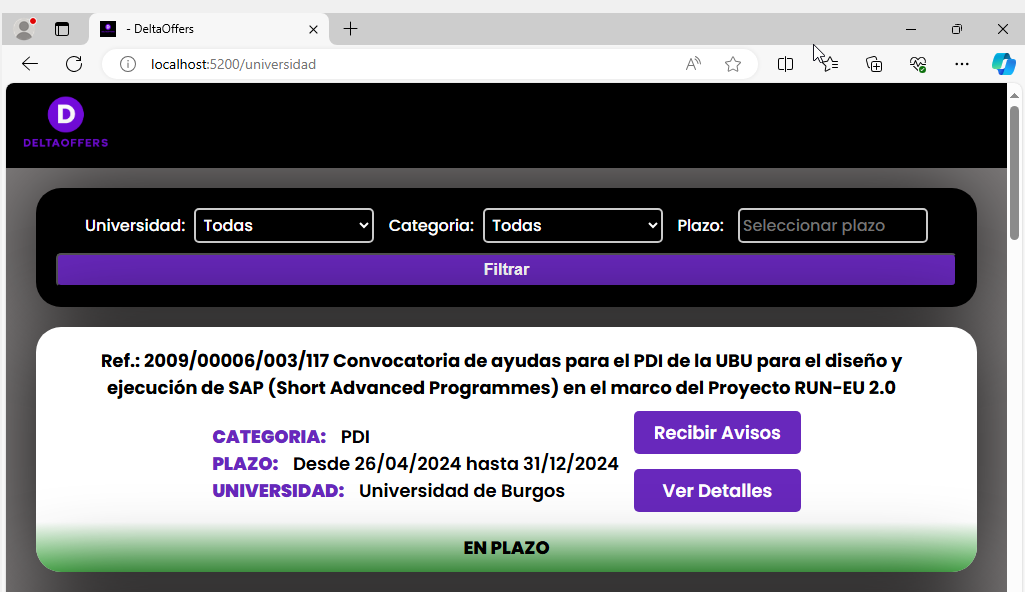
\includegraphics[width=1\linewidth]{DocumentacionTFG//img/WebLocal.PNG}
    \caption{Aplicación en .NET ejecutada en local}
\end{figure}

Para que el tribunal pueda probar el proyecto de manera local, se ha preparado una máquina virtual en la que se ha cargado el proyecto siguiendo los pasos previos. Esa máquina virtual será entregada al tribunal junto con la documentación y los directorios del proyecto en un USB.

\section{Pruebas del sistema}
Para asegurarnos que el software realizado fuese de calidad, se decidieron implementar pruebas unitarias al proceso de \textit{web scraping}. Gracias a la realización de test, pudimos percibir algunos errores que aparecían en el código de los cuales no era consciente a la hora de programar. 

Estos test fueron desarrollados con Python. Para ello, utilizamos la herramienta \textit{unittest} la cual permite la automatización de test, agregación de test en colecciones e independencia de los test de la estructura que los reporta.

Además, también se utilizó la herramienta  \textit{MagicMock} ~\cite{mock:latex}. Esta es una biblioteca cuya función es simular el comportamiento de otros objetos. De esta manera evitamos la utilización de los objetos para la realización de test unitarios de manera directa.

Algunas de las pruebas que se han realizado mediante la implementación de los test son las siguientes:

\begin{itemize}
    \item Comprobación de que el número de convocatorias obtenidas fuese el correcto.
    \item Comprobación de que el número de campos obtenido fuese correcto.
    \item Comprobación número mínimo de convocatorias
    \item Comprobación de que el número de convocatorias cerradas fuese correcto.
    \item Comprobación de que los campos tuviesen el valor y el formato deseado.
\end{itemize}

Para la ejecución de estas pruebas unitarias, en primer lugar, abriremos el proyecto en Python. Posteriormente, abriremos una nueva terminal en el proyecto y nos cambiaremos del directorio actual al directorio 'Test' . Finalmente, ejecutaremos lo siguiente: 

\begin{figure}[H]
    \centering
    \includegraphics[width=1\linewidth]{DocumentacionTFG//img/EjecuciónTest.PNG}
    \caption{Ejecución Test}
\end{figure}

Ejecutamos estos test con la opción \textit{-v} para que estos se ejecuten en modo \textit{verbose} y, por lo tanto, se nos proporcionará una mayor información de la prueba implementada y el resultado de la misma.

Por otro lado, para comprobar que la aplicación haya sido desarrollada correctamente, se implementaron pruebas manuales. Para la realización de estas pruebas, fui anotando los distintos escenarios o caminos que podría tener la web. Posteriormente, actué como '\textit{tester}' y fui comprobando que los resultados obtenidos en las diferentes ventanas de la aplicación eran los esperados.
